\chapter{Longest Chain Protocol Meets BFT}
Blockchain protocols must satisfy two basic properties: safety and liveness. They are jointly referred to as security properties.
For any given protocol, security properties cannot be guaranteed unconditionally. Naturally, we would like safety and liveness to hold under as large a set of conditions as possible; e.g., safety and liveness guarantees under $\frac{1}{2}$
honest majority would be preferable over these guarantees under $\frac{2}{3}$ honest majority.\\\\
One of the main advantages of the (Proof-of-Work) longest-chain protocol is that it operates in a fully permissionless setting. This means that it can handle changes in the number of participants; anyone can join or leave the system at any time. The crucial point here is that it remains secure even if only one participant is active (as long as the majority of the participants are honest at all times). This property is called adaptivity. However, the longest chain protocol also has some drawbacks. For instance, its safety guarantees are not deterministic, but probabilistic. Moreover, the protocol becomes insecure during periods of asynchrony, when the network delays are unpredictable. During such periods, the adversary can easily create many blocks and reverse blocks that are k-deep, thus breaking the safety of the k-deep confirmation rule. It also loses liveness.\\\\
We have learned about permissioned (committee-based) BFT protocols in the previous Chapters. These protocols provide deterministic safety (also known as finality). This means that the safety property is always preserved, even when the network is asynchronous for a long time. However, permissioned protocols have a limitation: they lack adaptivity. This means that the protocol will not make progress when the participation level is too low (but safety will never be violated).
\begin{figure}[h!]
	\centering
	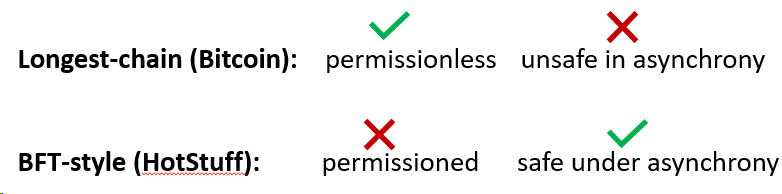
\includegraphics[width=0.4\linewidth]{Fig/17/F1}
	\caption{Two families of Blockchain protocols}
	\label{fig:L17_f1}
\end{figure}\\
We might wonder if we can design a blockchain protocol that has both features: finality and adaptivity.
We will explore how finality gadgets can help us create a blockchain system that has two different confirmation rules: one for adaptivity and one for finality. Finality gadgets are fascinating because they cleverly combine a BFT protocol with the longest-chain protocol, to make a protocol that has the best of both worlds. We will also talk about the CAP theorem, which shows us that it is impossible to have a single blockchain protocol that has both features.\\\\
There are other ways to compare the longest-chain protocol and the committee-based protocols, besides adaptivity and finality. One important factor is the latency in confirming blocks. The Nakamoto consensus protocol takes a long time to confirm blocks. You have to wait for the blocks to be k-deep before you can trust them. The blocks come at a rate that depends on the maximum network delay $\Delta$. So, the longest-chain protocol has a latency of $O(k\Delta)$.\\\\
We have seen how protocols like Prism can improve this to $O(\Delta)$. But protocols like HotStuff can do even better, with a latency of $O(\delta)$, where $\delta$ is the actual network delay (which can be much lower than the worst-case scenario). This property is called responsivity; the protocol adapts to the real network delay. Note that not all committee-based protocols are responsive, for example, Streamlet is not.\\\\
We might wonder if we can have a protocol that is responsive in a permissionless setting. This means that the protocol can confirm blocks quickly, even when anyone can join or leave the system. One way to achieve this is by using a protocol design called Hybrid Consensus, which cleverly combines a BFT protocol with the longest chain protocol.

\section{Hybrid Consensus}
The main goal of the Hybrid Consensus approach is to develop a Proof of Work permissionless system with fast confirmation.
In Algorand, which uses Proof of Stake, Verifiable Random Functions were used to select a committee, which then ran a fast-confirmation protocol. Inspired by Algorand, the main challenge is to choose a fixed-size committee in a PoW system, and also to do it periodically.\\\\
We will start by looking at how to choose one committee of size csize. We will run the Nakamoto consensus protocol until csize + k blocks are mined. Then all parties will agree on the first csize blocks (except with negligible probability). Each block has the miner’s public key in it. And there we have it, we have selected a group of csize nodes (or more precisely, csize public keys, which could belong to the same person or entity).\\\\
This committee is selected in a fair and decentralized way (because of PoW) and everyone agrees on it (because of the security of the PoW longest chain protocol). Once a committee is selected, it runs a fast and reliable BFT protocol (like HotStuff) to confirm transactions. So, the transactions are actually confirmed by the BFT protocol, not the longest-chain protocol.
\begin{figure}[h!]
	\centering
	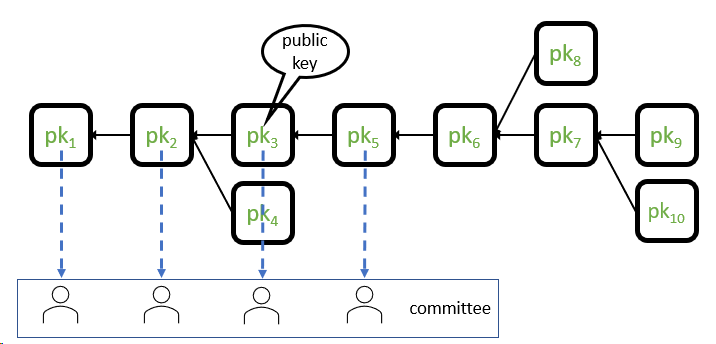
\includegraphics[width=0.6\linewidth]{Fig/17/F2}
	\caption{Hybrid Consensus}
	\label{fig:L17_f2}
\end{figure}\\
We will now look at the protocol in more detail. First of all, note that honest miners have to keep mining, even if they want to elect only one committee. Otherwise, the dishonest miners can make a longer chain with only dishonest blocks, which will then choose the committee. \\\\
Secondly, to run a fast and reliable BFT protocol like HotStuff, we need more than $\frac{2}{3}$ csize honest parties in the committee. This also depends on the ratio of honest and dishonest parties in the PoW protocol. In fact, if we use the simple longest chain protocol, we need a $\frac{3}{4}$ honest majority, because of the low quality of the chain. But, if we use FruitChains, we can do with a $\frac{2}{3}$ honest majority.\\\\
We need to change the committee regularly, for two reasons:
\begin{enumerate}
	\item we cannot expect the committee to stay online all the time for a long time.
	\item an adversary can bribe the committee after it is selected (but with some delay)
\end{enumerate}
By changing the committee often, we can prevent attacks by an adaptive adversary. The change is done in a simple way: once a committee is made, it keeps confirming transactions for a fixed amount of time, until the PoW blockchain grows by csize more blocks. When this happens, the old committee passes on the duty of transaction confirmation to the new committee. Note that everyone in the protocol sees the same committee.\\\\
The main advantage Hybrid Consensus brings over the longest-chain protocol is that it is a responsive protocol.\\
We will now look at some of the drawbacks of Hybrid Consensus.
\begin{itemize}
	\item  First of all, if we want a fast and reliable BFT protocol, the maximum fraction of dishonest parties it can handle is $\frac{1}{3}$, instead of $\frac{1}{2}$. This is unavoidable; any fast protocol can only deal with up to $\frac{1}{3}$ Byzantine adversaries. There are BFT protocols that can deal with up to $\frac{1}{2}$ adversaries, but their latency is $O(\Delta)$, which means that they depend on the maximum network delay.
	\item Another problem with Hybrid Consensus is that it does not work well under asynchrony, when the network delays are unpredictable. This is because the committee selection mechanism itself loses both safety and liveness. If there is no agreement on who is in the committee, there can be no agreement on the transactions confirmed by them. For the same reasons, the security of the whole system is not deterministic, but probabilistic.
	\item Another requirement for Hybrid Consensus is that honest committee members must stay active for the whole time that they are part of the committee. If too many of them stop participating, the protocol will stop working.
\end{itemize}
Thus, in terms of guaranteeing safety and liveness under a wide variety of conditions, Hybrid Consensus actually does worse than the longest-chain protocol. It does not guarantee liveness under variable participation.
	
	\section{The CAP Theorem}
	Finality and availability are two important properties of blockchain consensus protocols.
	\begin{itemize}
		\item \textbf{Finality} means that the transactions that are recorded on the blockchain are irreversible and cannot be changed or reverted by anyone. BFT protocol has this property.
		\item \textbf{Availability} means that the blockchain network can continue to operate and process transactions even when some nodes fail or leave. PoW longest chain has this property.
	\end{itemize}
	We might wonder if we can have a single ledger that has both adaptivity and finality. Sadly, this is impossible. The reason for this impossibility is a famous result in distributed systems, called the CAP theorem (CAP stands for Consistency, Availability and Partition tolerance).\\\\
	Roughly speaking, the CAP theorem states that during a network partition, a distributed system must make a choice between availability (liveness) and consistency (safety); it cannot offer both. Moreover, this choice must be encoded in its design itself.
	Thus, systems can be classified as availability favoring or consistency favoring, based on their design.\\\\
	The essence of the impossibility result is that it is difficult to distinguish network asynchrony from a reduced
	number of participants in the blockchain system. Hence, a protocol's behavior must be similar under both these conditions. 
	\begin{figure}[h!]
		\centering
		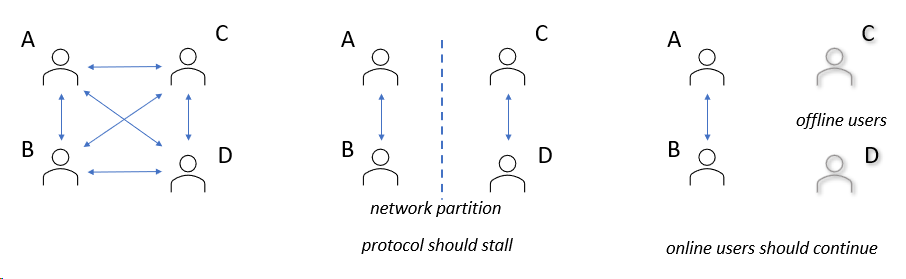
\includegraphics[width=0.6\linewidth]{Fig/17/F3}
		\caption{A decentralized protocol cannot distinguish between offline users and network partition
		}
		\label{fig:L17_f3}
	\end{figure}
	The CAP theorem also explains why there are two different kinds of protocols in the blockchain world. Protocols that use the longest-chain rule prefer liveness, which makes them adaptive. Protocols that use a committee of validators (like Hotstuff) prefer safety, which gives them finality.\\\\
	The CAP theorem lets users choose between adaptivity and finality, depending on their needs. We can use a special gadget that gives us two ways to confirm transactions: one that is adaptive, and one that is final. This way, users can decide locally which one they want to use. For example, if you are buying a coffee, you might not care about finality, and just want a fast confirmation. But if you are buying a Tesla, you might want to be sure that the transaction is final, and not risk it being reversed.
	\begin{figure}[h!]
		\centering
		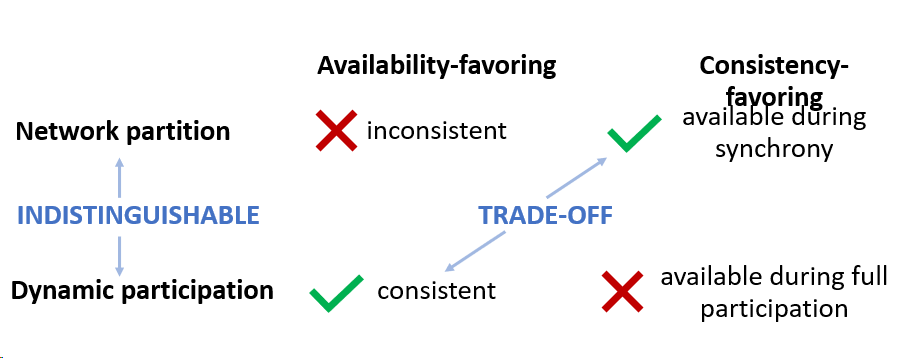
\includegraphics[width=0.5\linewidth]{Fig/17/F4}
		\caption{CAP Theorem in Blockchains}
		\label{fig:L17_f4}
	\end{figure}
	
	\subsection{Proof of CAP Theorem}
	We can show the CAP theorem with a simple example of a distributed system. Imagine there are two servers, $p_1$ and $p_2$. They both have a variable $V$ that has the value $x$ at first. Then, they get separated by a network problem. While they are separated, some client asks server $p_1$ to change $V$ to $y$. Now, $p_1$ has to decide what to do, and it has two options:
	\begin{itemize}
		\item It can say "ok" to the client and change $V$ to $y$. This means it is available, but $p_2$ still has $V$ as $x$. So, when another client asks either $p_1$ or $p_2$, they will get different answers, and the system is not consistent.
		\item It can wait for $p_2$ to come back online and not say "ok" to the client or change $V$. This means it is consistent, but not available, because it ignores the client.
	\end{itemize}
	\begin{figure}[h!]
		\centering
		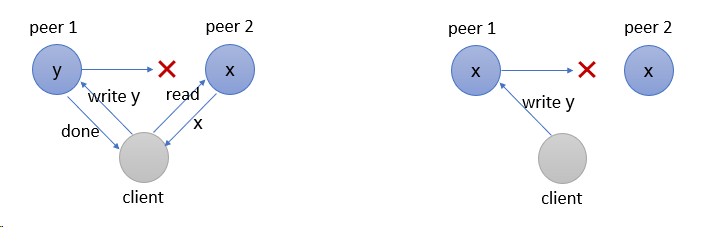
\includegraphics[width=0.7\linewidth]{Fig/17/F5}
		\caption{A visualization of the trade-offs implicated by the CAP theorem}
		\label{fig:L17_f5}
	\end{figure}
	$P_2$ also has to make the same trade-off when a client wants to read $V$. It should try to talk to $p_1$ to see whether $V$ has changed or not. But it can’t do that because of the network problem. It can either give an answer after some time (and risk giving the wrong answer) or never give an answer at all. So, if the network is slow and unpredictable (i.e., there is no limit on how long a message takes to reach), the system can’t have both consistency (correctness) and availability (responsiveness).
	\section{Finality Gadgets}	
	A finality gadget is a tool that adds finality to a PoW blockchain. Finality means that once a block is confirmed, it can’t be reversed. We want the blockchain to have finality and also adaptivity, which means it can adjust to changing conditions. To do this, we can combine two types of protocols: a longest-chain protocol and a BFT protocol. A longest-chain protocol is adaptive, but not final. A BFT protocol is final, but not adaptive. We want to get the best of both worlds, so we need to find a way to mix them together.
	
	\subsection{A two-layer design}
	In its simplest form, a finality gadget is a layer-two committee-based BFT protocol, which runs on top of a (layer-one) longest-chain protocol. One can use any adaptive protocol instead of the longest-chain protocol, but for this lecture, we shall focus on the longest-chain protocol. There are two sets of nodes in the system:
	\begin{itemize}
		\item \textbf{Miners} : Using PoW and the longest-chain rule, miners create new blocks that contain transactions. The number of miners can vary, but we assume that the system’s mining rate is stable.
		\item \textbf{Checkpointers} : Instead of creating any blocks themselves, the checkpointers run a BFT protocol that is based on a committee. They vote on the blocks that the PoW miners have created.
	\end{itemize}
	Therefor, to reach consensus on the same set of blocks (transactions), two consensus protocols run at the same time.
	\subsubsection{Checkpointing}
	Checkpointing is a new concept that we explain more here. Imagine that the longest chain protocol runs for a while, and the block tree reaches a certain height. Consider a block that has six blocks above it; a user could accept it, hoping that all future blocks would be its descendants. But the acceptance guarantee would be based on chance, as we know. How can we make the acceptance guarantee certain? In other words, how can we checkpoint this block?\\\\
	The checkpointing committee is responsible for checkpointing blocks, by giving checkpoint certificates for blocks. A checkpoint certificate for a block $B$ is a set of at least $\frac{2n}{3}$ signed messages of the form $<$finalized, B$>$; such a block is called checkpointed. These messages are part of almost all committee-based BFT protocols. Any node that gets this certificate can be sure that this block is confirmed for sure. This node could be a miner, a checkpointer, or just a watcher of the system. Of course, the checkpoint blocks, given by the second-level gadget, should be on the longest chain, to keep consistency with the first-level protocol. How can we make this happen?\\\\
	The checkpointers monitor the blocks that the miners create. At regular intervals, they run a (one-time) BFT protocol, where they input blocks that the miners have made. Honest nodes input blocks that are on the longest chain, but have not been checkpointed yet. Usually, blocks at a certain fixed depth are picked; for example, a depth of 6. This would make sure that if nodes have chains of the same length and have 6 blocks in common at the end, their inputs would be the same. Checkpointers vote on each other’s inputs, and finally decide on one specific input; this becomes the checkpointed block.
	\begin{figure}[h!]
		\centering
		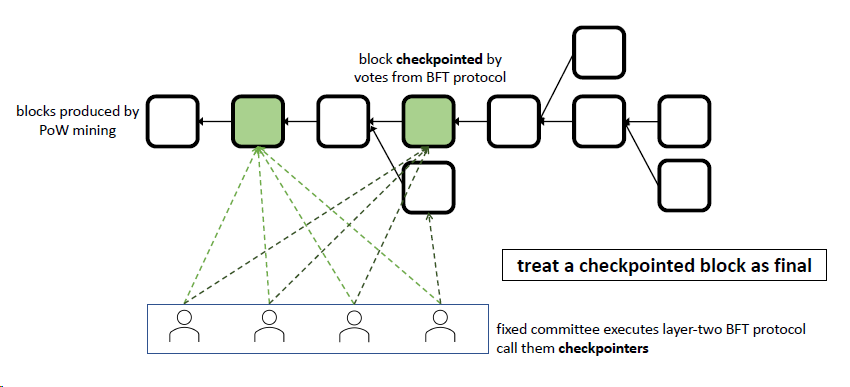
\includegraphics[width=0.6\linewidth]{Fig/17/F6}
		\caption{Finality Gadget}
		\label{fig:L17_f6}
	\end{figure}
	
	\subsection{Two ledgers and their properties.}
	A system that uses a finality gadget has two different confirmation rule:
	\begin{itemize}
		\item First, the k-deep rule is still a valid confirmation rule in the system, because blocks are mined according to the longest-chain protocol. A node that just watches the blocks mined in the system can easily follow this rule to confirm blocks. Such a node may remain completely oblivious to the checkpointing protocol. This rule provides adaptivity.
		\item The checkpointers also provide another way of confirming blocks, by giving checkpoint certificates for some blocks at regular intervals. This set of messages proves that block B has been chosen by the checkpointers. The confirmation rule for the finality gadget is to simply confirm the most recent checkpointed block, and all its ancestors. This rule provides finality.
	\end{itemize}
	Let’s see what adaptivity and finality mean for a confirmation rule. To do that, we need to keep in mind these points:
	\begin{enumerate}
		\item Every confirmation rule creates a ledger: it is the order of all transactions in the blocks confirmed by that rule.
		\item Over a long time, the two ledgers are the same: all transactions that are in one ledger are also in the other, and they have the same order.
		\item At any given time, one ledger could be slightly ahead of the other (i.e., confirm a few more transactions). Usually, we expect the k-deep rule (for small/moderate k) to confirm blocks faster than the checkpoint-based ledger. So, the ledger made by the k-deep rule will be a bit ahead of the checkpoint-based ledger.
	\end{enumerate}
	Under optimal conditions (i.e., static and synchronous), both ledgers grow at the same rate. Under variable participation, the finality-preserving ledger stalls, while the adaptive ledger keeps growing. As soon as static participation returns, the finality-preserving ledger catches up.
	
	\subsection*{Two confirmation rules}
	At first, it may seem strange to have more than one confirmation rule, but it makes sense if we think about it. In fact, the longest-chain protocol already has many confirmation rules! To see this better, let us separate the block production rule and the confirmation rule of the protocol. The block production rule is to make a new block at the end of the longest chain you have seen so far; this is the rule that gives the longest-chain protocol its name. The confirmation rule is to confirm a block that is k blocks deep, and all the blocks before it. All players follow the same block production rule. But, each user can pick their own confirmation rule, i.e., they each pick their own k value, depending on how much security they want and how much delay they can accept.
	
	\subsection*{Validity conditions}
	We need to be careful about how we pick the inputs for the BFT protocol and how we decide which inputs are valid. Some validity rules are needed, or else bad checkpointers could suggest random blocks for checkpointing, and these might get checkpointed. A validity rule would help honest nodes ignore invalid blocks. Choosing the right validity rules is a hard design problem. For example, we want checkpoints to be for fairly new blocks. Checkpointing an old block is not very useful, because it will already be confirmed with very high probability using the k-deep rule. But, we should not confirm a block very close to the end, because the longest-chain may change from there. Checkpointing a d-deep block, for some moderate value of d, is a possible compromise.
	
	\subsection*{Permissioned or Permissionless?}
	The checkpointers are a set of nodes that need permission to join in the current design. Can we make the checkpointing process open to anyone? In theory, they could be changed regularly from a large pool of players using a PoS method, like Algorand does. But, some degree of a permissioned system is unavoidable. A pure PoW system cannot give the finality properties we want (the best we could do was what Hybrid Consensus did, but that does not meet our needs). For simplicity, in this chapter, we just assume that the checkpointers stay the same for the whole protocol.
	
	\subsection{Examining Adaptivity and Finality}
	We wanted to use finality gadgets to combine a longest-chain protocol and a committee-based BFT protocol to get a system that has both adaptivity and finality. The system design gives us two ways of confirming blocks, and makes us think that the k-deep rule would give adaptivity, and the checkpoint-based rule would give finality. Let’s see if we really achieve this.\\\\
	The k-deep rule is adaptive in our two-layer design, because blocks are mined the same way as they are in the normal longest-chain protocol. The second-layer checkpointing protocol does not affect the first-layer protocol. How does the checkpointing protocol work under variable participation? If not enough checkpointers are active, the protocol simply stops. When all honest checkpointers are online again, they continue checkpointing blocks. So, under variable participation, the checkpointing protocol turns off and on for random periods, depending on how many checkpointers are participating. This only affects the liveness of the protocol; the safety is always preserved.\\\\
	We want to see if the finality gadget can protect the protocol when there is asynchrony. That means, even after a period of asynchrony, all blocks until the last checkpointed block should stay confirmed. We do not expect that any new blocks will be checkpointed in this period. When synchrony comes back, the protocol should resume checkpointing new blocks, and thus regain liveness. Is this requirement met by the design we have described?
	It does not work. Imagine a long period of asynchrony. The adversary can make a new chain that splits from before the last checkpointed block, and becomes the longest chain. When synchrony comes back, all miners will see the adversarial chain as the longest chain and will mine on that. There will be no new blocks after the last checkpointed block! At this point, the checkpointers have to either stop completely or (deliberately) break safety by changing chains. Both of these are bad.
	
	\subsection{checkpointed longest chain rule}
	This problem happens because we have a two-layer solution. This means that the checkpointers do not affect the miners’ behavior. For a finality gadget to work well, miners must follow the checkpointed blocks. In particular, miners should mine after the latest checkpointed block. Of course, we also want some longest-chain-like properties.\\\\
	A good idea is that miners follow the checkpointed longest chain rule: add to the longest chain after the latest checkpoint block. Since the latest checkpoint block is also the highest checkpoint block, this rule could also be said as: mine on the longest block that has all the checkpoint blocks. Under synchrony, all checkpoints would be on the longest chain by design. Following the checkpointed longest chain rule would be the same as following the longest chain rule. So, the new protocol would keep the security guarantees of the old protocol. \\\\
	On the other hand, the checkpoints protect the system during a long period of asynchrony. If the adversary mines blocks going back before the previous checkpoint, all honest nodes would simply ignore such blocks as invalid. For all practical purposes, every new checkpoint acts like a new starting point.\\\\
	We need to be careful about how we design the checkpointed longest-chain protocol, because the checkpointing protocol influences the miners. One vulnerability is how the checkpointing protocol behaves during variable participation. It is possible that the checkpointing protocol stops for a very long time, because of low participation. When participation comes back, we want the protocol to start checkpointing quickly, and close to the end of the longest chain. At all times, the protocol must make sure that the checkpoints are always on the longest chain. To do this, we need to pay special attention to the validity rules we mentioned before.